\documentclass[12pt,a4paper]{article}

\makeatletter
\def\input@path{{/home/maenwe/Master_CSM/modèle_cours_latex}}
\makeatother

\usepackage{prise_de_note}


\begin{document}
	
	
	\begin{titlepage}
		\centering
		
		% Logo
		\begin{figure}[h]
			\centering
			% Ajustez la largeur si besoin (ex: 0.4 ou 0.6)
			
\includegraphics[width=0.5\textwidth]{logo.jpg} 
		\end{figure}
		
		\vspace{2cm}
		
		% Filet horizontal du haut
		\rule{\linewidth}{0.5mm} \\[0.4cm]
		
		% Titre
		{\color{bleuTitre} \Huge \bfseries Cours} \\[0.4cm]
		
		% Filet horizontal du bas
		\rule{\linewidth}{0.5mm}
		
		\vspace{1.5cm}
		
		{\Large \textbf{Équation différentiels partiels}}
		
		\vfill
		
		% Bloc Informations
		\begin{minipage}{0.45\textwidth}
			\begin{flushleft} \large
				\textbf{Enseignant :} \\
				M. Eric \textsc{CASTELLAN}
			\end{flushleft}
		\end{minipage}
		\hfill
		\begin{minipage}{0.45\textwidth}
			\begin{flushright} \large
				\textbf{Étudiant :} \\
				Nathan \textsc{HASCOET}
			\end{flushright}
		\end{minipage}
		
		\vspace{2cm}
		
		% Date
		{\large \today}
		
	\end{titlepage}
	
	\section{Dynamique de $N$ particules en interaction}
	
	\fbox{\red !} $N$ particules identiques, décrites classiquement par les équations de Newton \fbox{\red !}\\
	On ne part pas des équations de Schrödinger. 
	
	Donnons nous la fonction $F(x)$ qui est la force d’interaction entre 2 particule, c'est-à-dire :
	
	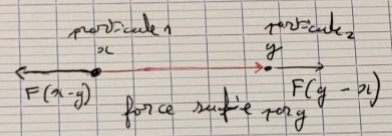
\includegraphics[scale = .5]{photo1.png}
	
	\begin{ex}[Attraction gravitationnelle]
		$ $
		\begin{center}
			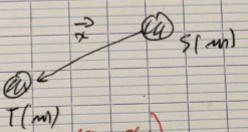
\includegraphics[scale = .5]{photo2.png}
		\end{center}
		
		\begin{minipage}{18cm}
			Force subie par la terre du fait du Soleil : $-G\dfrac{Mm}{\|x\\|^2}\dfrac{x}{\|x\|} = -\dfrac{GMm}{\|T-S\|^3}(T-S)$.\\
			
		Force subie par le Soleil du fait de la Terre : $-G\dfrac{Mm}{\|x\|^2}\dfrac{x}{\|x\|} = -\dfrac{GMm}{\|T-S\|^3}(T-S)$.
		\end{minipage}
		
		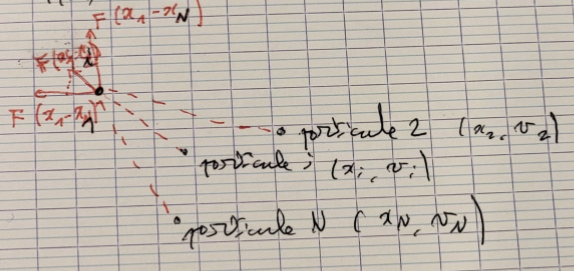
\includegraphics[scale = .5]{photo3.png}
	\end{ex}
	
	On a (Newton) :$\underbrace{\text{masse}}_{%
		\shortstack{\rouge{= 1, par soucis}\\\rouge{de normalisation}}%
	}$ $\times$ accélération = force pour toutes les particules
	
	particule 1 :  $\begin{cases}
		\frac{d^2x}{dt^2}(t) = T(x_1(t)-x_2(t)) + F(x_1(t)-x_3(t)) + \ldots + F(x_1(t) - x_N(t))\\
		\vdots \\
		\frac{d^2x_N}{dt^2}(t) = F(x_N(t)-x_1(t)) + F(x_N(t)-x_2(t)) + \ldots + F(x_N(t)-x_{N-1}(t)) 
	\end{cases}$
	
	\newpage
	
	Soit :\\
	$
	\begin{cases}
		\forall i = 1,...,N$, $\frac{d^2x_i(t)}{dt^2} = \displaystyle\sum_{\underbrace{j=1}_{j\not=i}}^N F(x_i(t) -x_j(t))\\
		\underline{\textcircled{+} \text{ données initiales à } t = 0}\\
		x_1(0) = x_1^0,\ldots,x_N^0(0) = x_N^0(0) \\
		v_1(0) = v_1^0,\ldots,v_N^0(0) = v_N^0(0)
	\end{cases}
	$
	
	avec $x_1^0,\ldots, x_N^0,$ positions initiales, données, chacune dans $\R^3$\\
	\hspace{1cm} $v_1^0,\ldots, v_N^0,$ vitesses initiales, données , chacune dans $\R^3$
	
	$\longrightarrow$ EDO d'ordre 2, en dimension $3N$ , avec typiquement, $N \simeq$ nombre d'Avogadro $\simeq 10^{23}$.\\
	\textbf{Calcul effectif inatteignable}.
	
	\par Cauchy-Lipschitz affirme que ce système admet une solution unique : d'où, $x_1(t),v_1(t),$ etc. sont entièrement déterminés par les données initiales.\\
	\textbf{\underline{Question :}} Que se passe t'il lorsque $N \to +\infty$ ?

	\par \underline{On a ici 2 limites naturelles :}\\
	\hspace*{2cm}\begin{minipage}[t]{18cm}
		\begin{enumerate}
			\item limite faible couplage (weak coupling limit) : hard sphere (sphère dure)\\
			Cas où les valeurs physique font que $F$ est de l'ordre de $\dfrac{1}{N}$, dans les unités physiquement pertinentes.\\
			On part alors de $\dfrac{d^2x_i}{dt^2}(t) = \dfrac1N \displaystyle\sum_{j\not = i} F(x_i(t)-x_j(t))$ et on passe à la limite $N \to \infty$
			\item limite faible densité (low density limit) : \\
			exemple typique de boule de billard de rayon $\epsilon$.
			
			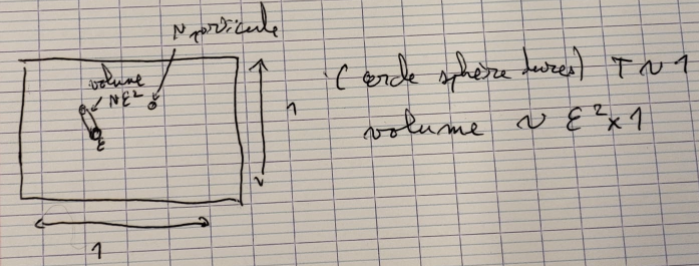
\includegraphics[scale = .5]{photo4.png}				
		
			On assure $N\epsilon^2 = 1$ ($N\epsilon^2 =$ sommes de valeurs explorés par chaque particule), ceci assure (à vue de nez au moins) que en temps 1 on a de l'ordre 1 collision.\\
			$\rightarrow$ Dans ce régime de convergence, on a convergence, lorsque $N \to +\infty$ vers l'équation de Boltzmann.
		\end{enumerate}
	\end{minipage}
	
	\rouge{Limite faible couplage}
	
	\vspace{-.2cm}
	
	On part de Newton.\\
	$\dfrac{d^2 x_i}{dt^2}(t) = \displaystyle\sum_{j=1}^F(x_i(t)-x_j(t))$ pour $i = 1,\ldots,N$ et $F$ connue, avec par exemple : $F(x) = -Gm^2\dfrac{x}{\|x\|^3}$,\\
	avec \begin{minipage}[t]{4cm}
			$x_i(0) = x_i^0$ connue.\\
			$v_i(0) = v_i^0$ connue.
		\end{minipage}
		\begin{minipage}[t]{10cm}
			\textbf{Soit $T$ l'ordre de grandeur de l'échelle temporelle}
		\end{minipage}
	
	\textbf{$X$ l'ordre de grandeur de l'échelle spatiale} (si le travail a été bien fait).\\
	les $v_i^0$ et les $v_i(t)$ vont demeurer de l'ordre de $\frac{X}{T}$.\\
	\textbf{Soit $\m F$ l'ordre de grandeur} de $F$.
	
	\underline{Introduisons la notation suivante :}\\
	\hspace{3cm} $X_N(t) = (x_1(t),\ldots,x_N(t)) \in \R^{3\times N}, X_N^0 = (x_1^0,\ldots,x_N^0)$.\\
	$V_N(t) = (v_1(t),,\ldots,v_N(t)) \in \R^{3\times N}, V_N^0 = (v_1^0,\ldots,v_N^0)$.\\
	$z_i(t) = (x_i(t),v_i(t)) \in \R^6$ (variable de l'espace des phases).\\
	$z_i^0 = (x_i^0,v_i^0)$.\\
	$Z_N(t) = (z_1(t),\ldots,z_N(t))\in\R^{6\times N}, Z_N^0 = (z_1^0,\ldots,z_N^0)$\\
	Avec ces notations, les équations de Newton s'écrivent :
	\begin{center}
		
	$\begin{cases}
		m \dfrac{d^2 X_N}{dt^2}(t) = f(X_N(t)) \text{ où } f : \alpha \mapsto \left(\displaystyle\sum_{\underset{j\not = 1}{j=1}}^N F(\alpha_1-\alpha_j),\ldots,\sum_{\underset{j\not = N}{j=1}}^N F(\alpha_N-\alpha_j)\right)\\
		X_N(0) = X_N^0, V_N(0) = V_N^0
	\end{cases}$
	\end{center}
	
	\underline{Adimensionnons ce système :}\\
	Posons $t = T \overset{\sim}{t}$ \hspace{1cm} \begin{minipage}[t]{4 cm}
														où $\overset{\sim}{t}$  est d'ordre $1$ et $\overset{\sim}{t}$  est sans dimension.
													\end{minipage}\\		
	$x_i(t) = X\overset{\sim}{t}\left(\frac{t}{T}\right)$
	
	De manière équivalente, on pose : $x_n(T) = x\overset{\sim}{X}_N\left(\frac{t}{T}\right)$.\\
	$\overset{\sim}{X}_N(\m F) = \dfrac{X_N(T\m F)}{X}$\\
	Soit $\overset{\sim}{V}_N(\m F) = \dfrac{d \overset{\sim}{X}_N(t)}{d\overset{\sim}{t}} = \dfrac{T}{X} V_N(T\m F)$
	
	\par Enfin, pour ce qui concerne le champ de force, on définit : $\begin{aligned}[t]
		\overset{\sim}{f}(\overset{\sim}{\alpha}) 
		&= \dfrac{f(X\overset{\sim}{\alpha})}{\m F} \\
		&= \left(\displaystyle\sum_{\underset{i\not=1}{i=1}}^N \dfrac{F(X(\overset{\sim}{\alpha}_i-\overset{\sim}{\alpha}_j))}{\m F}, \cdots \right)
	\end{aligned}$
	
	Ainsi partant de :
	\[
	m\dfrac{d^2X_N(t)}{dt^2} = f(X_N(t))
	\]
	
	On obtient, pour $\overset{\sim}{X}(\overset{\sim}{t}) = \dfrac{X_N(T\m F)}{X}$, la relation :
	\[
	\begin{aligned}[t]
		\dfrac{d^2\overset{\sim}{X}_N(t)}{d\overset{\sim}{t}^2} 
		&= \dfrac{T^2}{X}\left(T\m F\right) \\
		&= \dfrac{T^2}{X}\frac{1}{m}f(X_N(T\m F)) \\
		&= \dfrac{T^2\m F}{Xm} \overset{\sim}{f}(\overset{\sim}{X}_N(\m F))
	\end{aligned}
	\]
	
	c'est-à-dire : $\dfrac{d^2\overset{\sim}{X}_N(\overset{\sim}{t})}{d\overset{\sim}{t}^2} = \dfrac{T^2\m F}{X_m} \overset{\sim}{f}(\overset{\sim}X_N)$
	
	\fbox{+} $\overset{\sim}X_N(0) = \overset{\sim}X_N^0$, $\overset{\sim}{V}_N(0) = \overset{\sim}V_N^0$ \hspace{1cm} \fbox{+} $\overset{\sim}f(\overset{\sim}\alpha) = \left(\displaystyle\sum_{\underset{j\not = 1}{j=1}} \frac{F(X(\overset{\sim}\alpha_1-\overset{\sim}\alpha_j))}{\m F}, \cdots\right)$
	
	\fbox{Nous faisons désormais l'hypothèse que $\dfrac{T^2\m F}{X_m}$ est de l'ordre de $\dfrac{1}{N}$.}
	
	\par Partons des équations de Newton adimensionnées (en laissant tomber les tildes).
	\[
	\dfrac{d^2X_N}{dt^2}(t) = \dfrac{1}{N}G(X_N(t))
	\]
	où $G : \alpha \in \R^{3 \times N} \mapsto G(\alpha) = \left(\displaystyle\sum_{\underset{j\not = 1}{j=1}}^N F(x_1-x_j),\ldots,\sum_{\underset{j\not = N}{j=1}}^N F(\alpha_N-\alpha_j)\right)$\\ 
	et $F : \R^3 \to \R^3$ de classe $\m C^k$ avec $k \geq 1$.
	
	\par On souhaite procéder à la limite $N \to \infty$ dans ces équations (EDO en dimesion $3\times $ (gros problème topologiqueà, non linéaires)).\\
	\underline{\textbf{Idée profonde :}} au lieu de se donner un jeu de données inutiles dons notre équation de Newton, on se donne une fonction $f^0(x_1^0,v_1^0,x_2^0,v_2^0,\ldots,x_N^0,v_N^0)$, dite fonction de répartition (ou fonction de densité) qui permet de dire :
	
	\[
	\mathbb{P}\left(x_1^0\in \Omega_1,v_1^0 \in O_1,\ldots,x_N^0 \in Omega_N,v_N^0\in O_n \right) = \displaystyle\underset{\Omega_1\times O_1\times\cdots\times\Omega_N\times O_N}{\int}f^0(x_1^0,v_1^0,\ldots,x^0_N,v^0_N) dx_1^0dv_1^0\cdots dx_N^0dv_N^0
	\]
	
	\underline{Affirmation :} La fonction de répartition $f(t,x_1,t_1,\ldots,x_N,t_N)$
	
	\textbf{ENCOPE A COPIER}
	
\end{document}